\documentclass[a4paper,11pt]{article}
\usepackage{amsmath}
\usepackage{amssymb}
\usepackage[polish]{babel}
\usepackage{polski}
\usepackage[utf8]{inputenc}
\usepackage{indentfirst}
\usepackage{geometry}
\usepackage{array}
\usepackage[pdftex]{color,graphicx}
\usepackage{subfigure}
\usepackage{afterpage}
\usepackage{setspace}
\usepackage{color}
\usepackage{wrapfig}
\usepackage{listings}
\usepackage{datetime}

\renewcommand{\onehalfspacing}{\setstretch{1.6}}

\geometry{tmargin=2.5cm,bmargin=2.5cm,lmargin=2.5cm,rmargin=2.5cm}
\setlength{\parindent}{1cm}
\setlength{\parskip}{0mm}

\newenvironment{lista}{
\begin{itemize}
  \setlength{\itemsep}{1pt}
  \setlength{\parskip}{0pt}
  \setlength{\parsep}{0pt}
}{\end{itemize}}

\newcommand{\linia}{\rule{\linewidth}{0.4mm}}

\definecolor{lbcolor}{rgb}{0.95,0.95,0.95}
\lstset{
    backgroundcolor=\color{lbcolor},
    tabsize=4,
  language=C++,
  captionpos=b,
  tabsize=3,
  frame=lines,
  numbers=left,
  numberstyle=\tiny,
  numbersep=5pt,
  breaklines=true,
  showstringspaces=false,
  basicstyle=\footnotesize,
  identifierstyle=\color{magenta},
  keywordstyle=\color[rgb]{0,0,1},
  commentstyle=\color{Darkgreen},
  stringstyle=\color{red}
  }

\begin{document}

\noindent
\begin{tabular}{|c|p{11cm}|c|} \hline 
L2 & Przemysław Kleszcz, Krzysztof Tatar & \ddmmyyyydate\today \tabularnewline
\hline 
\end{tabular}


\section*{Zadanie 6 - Liczby pierwsze w CUDA}

Celem zadania było napisanie programu, który testuje podane duże liczby pierwsze. Do poprawnego działania programu należy podać jeden argument wejściowy \emph{primes - ścieżka do pliku z liczbami pierwszym}. Poniżej zaprezentowano główną funkcje programu odpowiedzialną za zrównoleglanie obliczeń.


\begin{lstlisting}
__global__ void prime(long long int* numbers, int* results)
{
	unsigned int numberIndex = blockIdx.x;
	unsigned long long int number = numbers[numberIndex];
	long long j;
	unsigned long long int sqrtNumber = rint(sqrt((double)number));
	
	__shared__ 
	bool flag;
	flag = false;

	__syncthreads();
	for (j = (threadIdx.x * (sqrtNumber / blockDim.x) + 2); j < (threadIdx.x * (sqrtNumber / blockDim.x)) + (sqrtNumber / blockDim.x) + 2; j++)
	{
		__syncthreads();
		if (flag)
			continue;

		if (number % j == 0)
		{
			flag = true;
			results[numberIndex] = 0;
		}
	}

	if (!flag)
		results[numberIndex] = 1;
}
\end{lstlisting}

Powyższy program sprawdza czy liczba jest pierwszą czy nie jest liczbą pierwszą. Do zrealizowania zadania został użyty podział na bloki oraz na wątki. Każdy blok sprawdza swoją liczbę czy jest pierwszą.
\newline
Główne funcje CUDA
\begin{lstlisting}
 __global__
\end{lstlisting}
Kwalifikator \_\_global\_\_to dodatek pochodzący z języka CUDA C. Informuje on kompilator
o tym, że dana funkcja powinna zostać skompilowana dla urządzenia, a nie dla hosta. 
\newline
\begin{lstlisting}
__shared__
\end{lstlisting}
Deklaracja zmiennej w pamięci wspólnej.
\newline
\begin{lstlisting}
unsigned int numberIndex = blockIdx.x;
\end{lstlisting}
blockIdx zawiera ona indeks bloku, który aktualnie wykonuje dany kod urządzenia.
\newline
\begin{lstlisting}
blockDim.x
\end{lstlisting}
W powyższym przypisaniu użyta została nowa zmienna wbudowana o nazwie blockDim. Jej
wartość jest stała w każdym bloku i reprezentuje liczbę wątków w każdym wymiarze bloku. Ponieważ nasz blok jest jednowymiarowy, używamy tylko odwołań bl ockDim.x.
\newline
\begin{lstlisting}
__syncthreads();
\end{lstlisting}
Najpierw muszą zakończyć się wszystkie operacje wątków znajdujące się w kodzie przed wywołaniem funkcji\_\_syncthreads(), a dopiero potem mogą być wykonywane dalsze instrukcje wątkowe.

\begin{lstlisting}
	cudaEvent_t timeStart, timeEnd;
	float time;
	cudaEventCreate(&timeStart);
	cudaEventCreate(&timeEnd);
	cudaEventRecord(timeStart, 0);
	prime<<<vecOfStr.size(),BLOCK_SIZE>>>(devNumbers, devResults);
	cudaDeviceSynchronize();
	cudaEventRecord(timeEnd, 0);
	cudaEventSynchronize(timeEnd);
	cudaEventElapsedTime(&time, timeStart, timeEnd);
\end{lstlisting}
Aby zmierzyć czas wykonywania bloku kodu, musimy utworzyć zdarzenie zarówno początku, jak
i końca. Najpierw nakażemy systemowi zarejestrować moment rozpoczęcia operacji, następnie damy
mu jakieś zadania do wykonania przez GPU, a na koniec zażądamy zakończenia rejestracji.
\begin{lstlisting}
	cudaFree(devNumbers);
	cudaFree(devResults);
\end{lstlisting}
Uwalnia przestrzeń pamięci wskazywaną przez wskaźnik.

\begin{lstlisting}
cudaMalloc((void**)&devResults, vecOfStr.size() * sizeof(int));
\end{lstlisting}
cudaMalloc alokuje pamięć na urzą­
dzeniu za pośrednictwem systemu wykonawczego CUDA.
\begin{lstlisting}
cudaMemcpy(results, devResults, vecOfStr.size() * sizeof(int), cudaMemcpyDeviceToHost);
\end{lstlisting}
Dodatkowo dostęp do pamięci urządzenia na hoście można uzyskać za pomocą funkcji
cudaMemcpy().
\begin{figure}[ht]
	\centering
  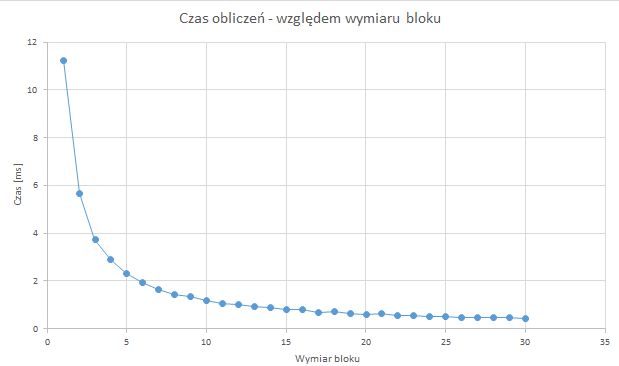
\includegraphics[width=0.7\textwidth]{2.png}
  \caption{Wykres przyspieszenia}
\end{figure}

Z powyższego rysunku można wywnioskować, że średni czas obliczeń dynamicznie malał dla pierwszych 10 bloków. Następnie dla. Następnie od 11 do 30 czas również stopniowo spada.

\end{document}
